\documentclass[english]{SPFShortReport}
\usepackage{subfigure}
\usepackage{spfFigures}
\usepackage{longtable}
\usepackage{url}
\usepackage{gensymb}
\usepackage[yyyymmdd,hhmmss]{datetime}
\reportName{Python calculation for heat pump SI-242}
\reportSubName{Parametric Heat Pump calculation} 
\reportDate{\today \hspace{0.1cm} at: \currenttime \hspace{0.1cm} h} 
\author{Dani Carbonell}
\address{dani.carbonell@solarenergy.ch}
\begin{document}
\begin{table}[!ht]
\begin{small}
\caption{Fitted coefficients for the heat pump.}
\begin{center}
\resizebox{12cm}{!} 
{
\begin{tabular}{l | c c } 
\hline
\hline
Coefficient &Description & \\ 
 & &$[kW]$\\ 
\hline
$PQ_{1}$ & \emph{$1^{st}$ condenser polynomial coefficient}  & 8.6790e+01    \\ 
$PQ_{2}$ & \emph{$2^{st}$ condenser polynomial coefficient}  & 9.3917e+02    \\ 
$PQ_{3}$ & \emph{$3^{st}$ condenser polynomial coefficient}  & -4.6678e+02    \\ 
$PQ_{4}$ & \emph{$4^{st}$ condenser polynomial coefficient}  & -4.4486e+03    \\ 
$PQ_{5}$ & \emph{$5^{st}$ condenser polynomial coefficient}  & 3.3440e+03    \\ 
$PQ_{6}$ & \emph{$6^{st}$ condenser polynomial coefficient}  & 1.2445e+03    \\ 
\hline
$PCOP_{1}$ & \emph{$1^{st}$ COP polynomial coefficient}  & 2.3058e+00    \\ 
$PCOP_{2}$ & \emph{$2^{st}$ COP polynomial coefficient}  & 1.3236e+02    \\ 
$PCOP_{3}$ & \emph{$3^{st}$ COP polynomial coefficient}  & 5.9440e+01    \\ 
$PCOP_{4}$ & \emph{$4^{st}$ COP polynomial coefficient}  & -6.7673e+02    \\ 
$PCOP_{5}$ & \emph{$5^{st}$ COP polynomial coefficient}  & 2.7135e+02    \\ 
$PCOP_{6}$ & \emph{$6^{st}$ COP polynomial coefficient}  & -3.2856e+02    \\ 
\hline
$\dot m_{cond}$ & 5400.00 $[kg/h]$\\ 
$\dot m_{evap}$ & 5400.00 $[kg/h]$\\ 
\hline
$COP_{nom}$ (B0W35)& 4.23 \\ 
$Q_{c,nom}$ (B0W35)& 45.26 kW\\ 
$COP_{nom}$ (B2W35)& 4.56 \\ 
$Q_{c,nom}$ (B2W35)& 47.79 kW\\ 
$COP_{nom}$ (B10W35)& 6.15 \\ 
$Q_{c,nom}$ (B10W35)& 60.90 kW\\ 
\hline
\hline
\end{tabular}
}
\label{CoefTable}
\end{center}
\end{small}
\end{table}
\begin{table}[!ht]
\begin{small}
\caption{Predicting results of the heat pump.}
\begin{center}
\resizebox{12cm}{!} 
{
\begin{tabular}{l | c c c c c c c c c c c } 
\hline
\hline
$T_{evap,in}$ &$T_{evap,out}$ &$T_{cond,in}$ &$T_{cond,out}$ &$COP$ &$Q_{cond}$ &$Q_{evap}$ &$W_{comp}$ &$\dot m_{cond}$ &$\dot m_{evap}$ &$\Delta T_{evap}$ &$\Delta T_{cond}$ \\ 
$^oC$ &$^oC$ &$^oC$ &$^oC$ &$[-]$ &$[kW]$ &$[kW]$ &$[kW]$ &kg/h &kg/h &K &K\\ 
\hline
-7.00 & -11.65 & 23.68 & 30.00 & 3.04 & 39.69 & 26.64 & 13.05 & 5400 & 5400 & 4.7 & 6.3\\ 
-7.00 & -11.70 & 32.59 & 38.75 & 3.28 & 38.71 & 26.90 & 11.81 & 5400 & 5400 & 4.7 & 6.2\\ 
-7.00 & -11.57 & 41.09 & 47.50 & 2.85 & 40.28 & 26.14 & 14.14 & 5400 & 5400 & 4.6 & 6.4\\ 
-7.00 & -10.28 & 49.27 & 56.25 & 1.75 & 43.88 & 18.78 & 25.10 & 5400 & 5400 & 3.3 & 7.0\\ 
-7.00 & -1.35 & 57.83 & 65.00 & 0.58 & 45.06 & -32.34 & 77.40 & 5400 & 5400 & -5.6 & 7.2\\ 
-4.00 & -9.35 & 23.19 & 30.00 & 3.52 & 42.77 & 30.61 & 12.16 & 5400 & 5400 & 5.3 & 6.8\\ 
-4.00 & -9.08 & 32.32 & 38.75 & 3.57 & 40.41 & 29.10 & 11.31 & 5400 & 5400 & 5.1 & 6.4\\ 
-4.00 & -8.67 & 41.05 & 47.50 & 2.93 & 40.57 & 26.71 & 13.85 & 5400 & 5400 & 4.7 & 6.5\\ 
-4.00 & -6.76 & 49.44 & 56.25 & 1.58 & 42.82 & 15.80 & 27.02 & 5400 & 5400 & 2.8 & 6.8\\ 
-4.00 & 50.24 & 54.62 & 65.00 & 0.17 & 65.25 & -310.46 & 375.72 & 5400 & 5400 & -54.2 & 10.4\\ 
-1.00 & -7.12 & 22.60 & 30.00 & 4.04 & 46.53 & 35.03 & 11.51 & 5400 & 5400 & 6.1 & 7.4\\ 
-1.00 & -6.58 & 31.94 & 38.75 & 3.93 & 42.83 & 31.92 & 10.91 & 5400 & 5400 & 5.6 & 6.8\\ 
-1.00 & -5.91 & 40.88 & 47.50 & 3.08 & 41.61 & 28.08 & 13.52 & 5400 & 5400 & 4.9 & 6.6\\ 
-1.00 & -3.52 & 49.46 & 56.25 & 1.51 & 42.65 & 14.43 & 28.21 & 5400 & 5400 & 2.5 & 6.8\\ 
-1.00 & 47.41 & 54.59 & 65.00 & 0.19 & 65.44 & -277.12 & 342.56 & 5400 & 5400 & -48.4 & 10.4\\ 
2.00 & -4.98 & 21.89 & 30.00 & 4.62 & 50.96 & 39.94 & 11.02 & 5400 & 5400 & 7.0 & 8.1\\ 
2.00 & -4.18 & 31.44 & 38.75 & 4.34 & 45.95 & 35.37 & 10.58 & 5400 & 5400 & 6.2 & 7.3\\ 
2.00 & -3.28 & 40.60 & 47.50 & 3.29 & 43.38 & 30.21 & 13.17 & 5400 & 5400 & 5.3 & 6.9\\ 
2.00 & -0.60 & 49.36 & 56.25 & 1.52 & 43.29 & 14.86 & 28.42 & 5400 & 5400 & 2.6 & 6.9\\ 
2.00 & 44.62 & 54.55 & 65.00 & 0.21 & 65.66 & -243.98 & 309.64 & 5400 & 5400 & -42.6 & 10.4\\ 
5.00 & -2.93 & 21.08 & 30.00 & 5.26 & 56.06 & 45.39 & 10.66 & 5400 & 5400 & 7.9 & 8.9\\ 
5.00 & -1.89 & 30.83 & 38.75 & 4.82 & 49.76 & 39.43 & 10.33 & 5400 & 5400 & 6.9 & 7.9\\ 
5.00 & -0.77 & 40.20 & 47.50 & 3.58 & 45.87 & 33.06 & 12.81 & 5400 & 5400 & 5.8 & 7.3\\ 
5.00 & 2.04 & 49.15 & 56.25 & 1.61 & 44.65 & 16.96 & 27.70 & 5400 & 5400 & 3.0 & 7.1\\ 
5.00 & 41.88 & 54.51 & 65.00 & 0.24 & 65.94 & -211.10 & 277.05 & 5400 & 5400 & -36.9 & 10.5\\ 
8.00 & -0.98 & 20.17 & 30.00 & 5.94 & 61.79 & 51.39 & 10.40 & 5400 & 5400 & 9.0 & 9.8\\ 
8.00 & 0.29 & 30.12 & 38.75 & 5.35 & 54.24 & 44.11 & 10.13 & 5400 & 5400 & 7.7 & 8.6\\ 
8.00 & 1.61 & 39.69 & 47.50 & 3.93 & 49.06 & 36.59 & 12.47 & 5400 & 5400 & 6.4 & 7.8\\ 
8.00 & 4.44 & 48.82 & 56.25 & 1.77 & 46.69 & 20.38 & 26.31 & 5400 & 5400 & 3.6 & 7.4\\ 
8.00 & 39.20 & 54.45 & 65.00 & 0.27 & 66.29 & -178.59 & 244.88 & 5400 & 5400 & -31.2 & 10.5\\ 
11.00 & 0.88 & 19.16 & 30.00 & 6.68 & 68.16 & 57.95 & 10.21 & 5400 & 5400 & 10.1 & 10.8\\ 
11.00 & 2.37 & 29.30 & 38.75 & 5.95 & 59.38 & 49.40 & 9.98 & 5400 & 5400 & 8.6 & 9.4\\ 
11.00 & 3.88 & 39.08 & 47.50 & 4.36 & 52.93 & 40.78 & 12.14 & 5400 & 5400 & 7.1 & 8.4\\ 
11.00 & 6.67 & 48.40 & 56.25 & 2.01 & 49.35 & 24.77 & 24.58 & 5400 & 5400 & 4.3 & 7.9\\ 
11.00 & 36.61 & 54.38 & 65.00 & 0.31 & 66.74 & -146.58 & 213.32 & 5400 & 5400 & -25.6 & 10.6\\ 
14.00 & 2.63 & 18.04 & 30.00 & 7.46 & 75.15 & 65.07 & 10.07 & 5400 & 5400 & 11.4 & 12.0\\ 
14.00 & 4.34 & 28.38 & 38.75 & 6.61 & 65.17 & 55.30 & 9.86 & 5400 & 5400 & 9.7 & 10.4\\ 
14.00 & 6.03 & 38.36 & 47.50 & 4.85 & 57.47 & 45.62 & 11.85 & 5400 & 5400 & 8.0 & 9.1\\ 
14.00 & 8.78 & 47.87 & 56.25 & 2.31 & 52.65 & 29.88 & 22.77 & 5400 & 5400 & 5.2 & 8.4\\ 
14.00 & 34.14 & 54.29 & 65.00 & 0.37 & 67.33 & -115.27 & 182.60 & 5400 & 5400 & -20.1 & 10.7\\ 
17.00 & 4.29 & 16.84 & 30.00 & 8.30 & 82.73 & 72.76 & 9.97 & 5400 & 5400 & 12.7 & 13.2\\ 
17.00 & 6.20 & 27.36 & 38.75 & 7.32 & 71.58 & 61.80 & 9.78 & 5400 & 5400 & 10.8 & 11.4\\ 
17.00 & 8.08 & 37.53 & 47.50 & 5.41 & 62.66 & 51.08 & 11.58 & 5400 & 5400 & 8.9 & 10.0\\ 
17.00 & 10.79 & 47.25 & 56.25 & 2.69 & 56.58 & 35.53 & 21.05 & 5400 & 5400 & 6.2 & 9.0\\ 
17.00 & 31.85 & 54.16 & 65.00 & 0.44 & 68.13 & -84.98 & 153.11 & 5400 & 5400 & -14.8 & 10.8\\ 
20.00 & 5.85 & 15.54 & 30.00 & 9.18 & 90.91 & 81.00 & 9.90 & 5400 & 5400 & 14.2 & 14.5\\ 
20.00 & 7.96 & 26.24 & 38.75 & 8.09 & 78.62 & 68.90 & 9.72 & 5400 & 5400 & 12.0 & 12.5\\ 
20.00 & 10.02 & 36.60 & 47.50 & 6.04 & 68.49 & 57.15 & 11.35 & 5400 & 5400 & 10.0 & 10.9\\ 
20.00 & 12.72 & 46.52 & 56.25 & 3.14 & 61.15 & 41.65 & 19.50 & 5400 & 5400 & 7.3 & 9.7\\ 
20.00 & 29.81 & 53.98 & 65.00 & 0.55 & 69.25 & -56.17 & 125.42 & 5400 & 5400 & -9.8 & 11.0\\ 
\hline
\hline
\end{tabular}
}
\label{ResultsTable}
\end{center}
\end{small}
\end{table}
\begin{figure}[!ht]
\begin{center}
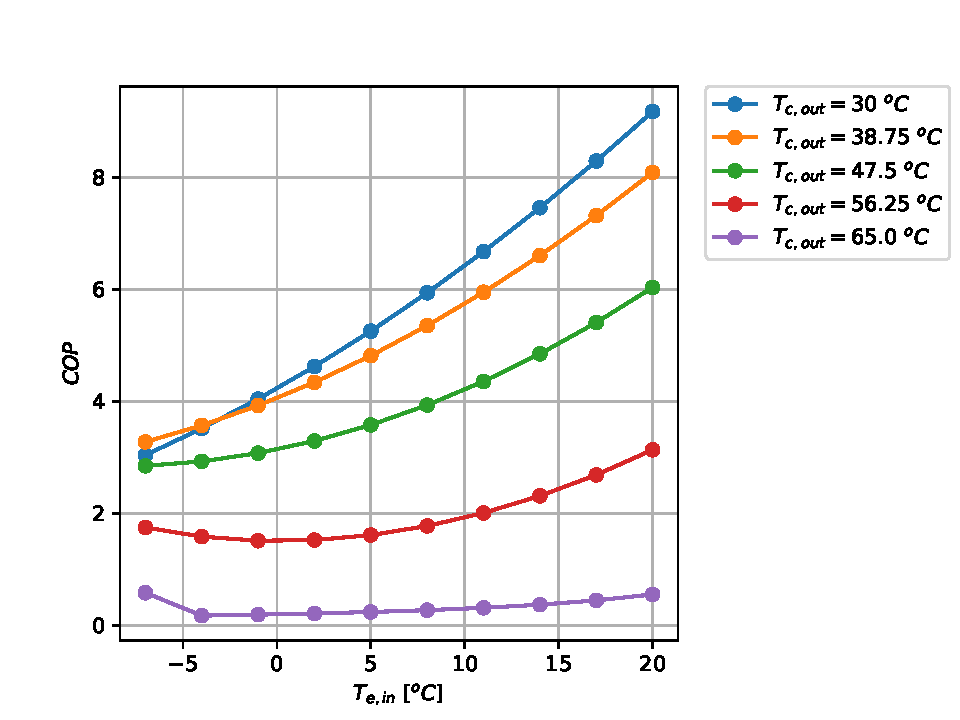
\includegraphics[width=1\textwidth]{C:/Daten/spfPackages/GIT/spfTrnsysFiles/HeatPump/BrineToWater/Walter Meier/SI-242/SI-242-Cop.pdf}
\caption{COP Results for the heat pump at the selected points}
\label{COPFig}
\end{center}
\end{figure}
\begin{figure}[!ht]
\begin{center}
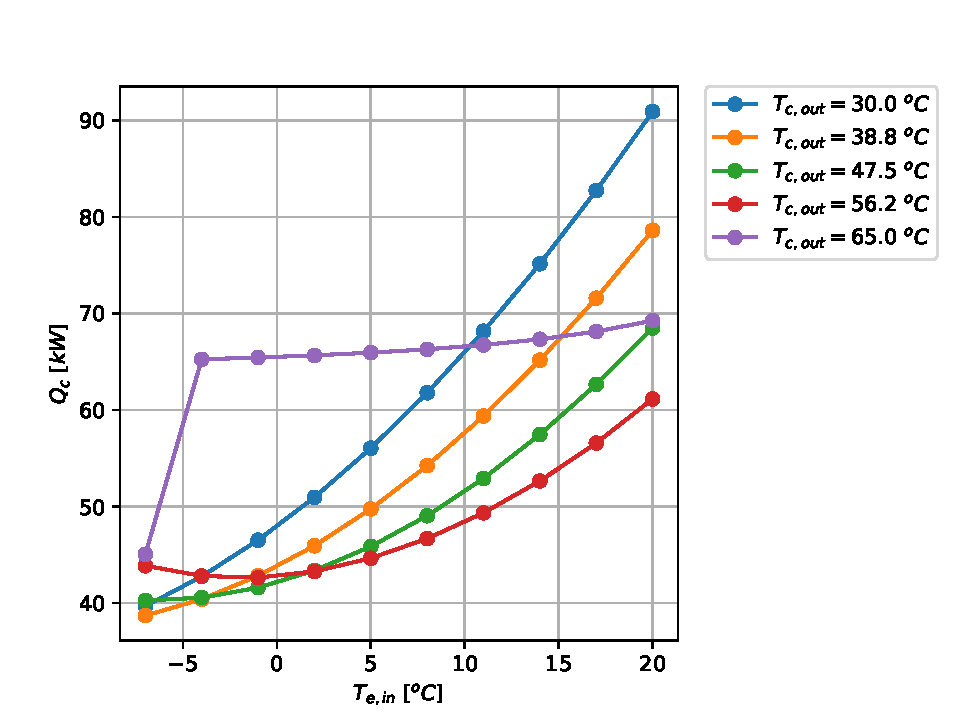
\includegraphics[width=1\textwidth]{C:/Daten/spfPackages/GIT/spfTrnsysFiles/HeatPump/BrineToWater/Walter Meier/SI-242/SI-242-Qc.pdf}
\caption{$Q_c$ Results for the heat pump at the selected points}
\label{QcFig}
\end{center}
\end{figure}
\end{document}
